\documentclass{standalone}
\usepackage{pgf}
\usepackage{tikz}
\usetikzlibrary{arrows,automata}
\usepackage[latin1]{inputenc}
\begin{document}
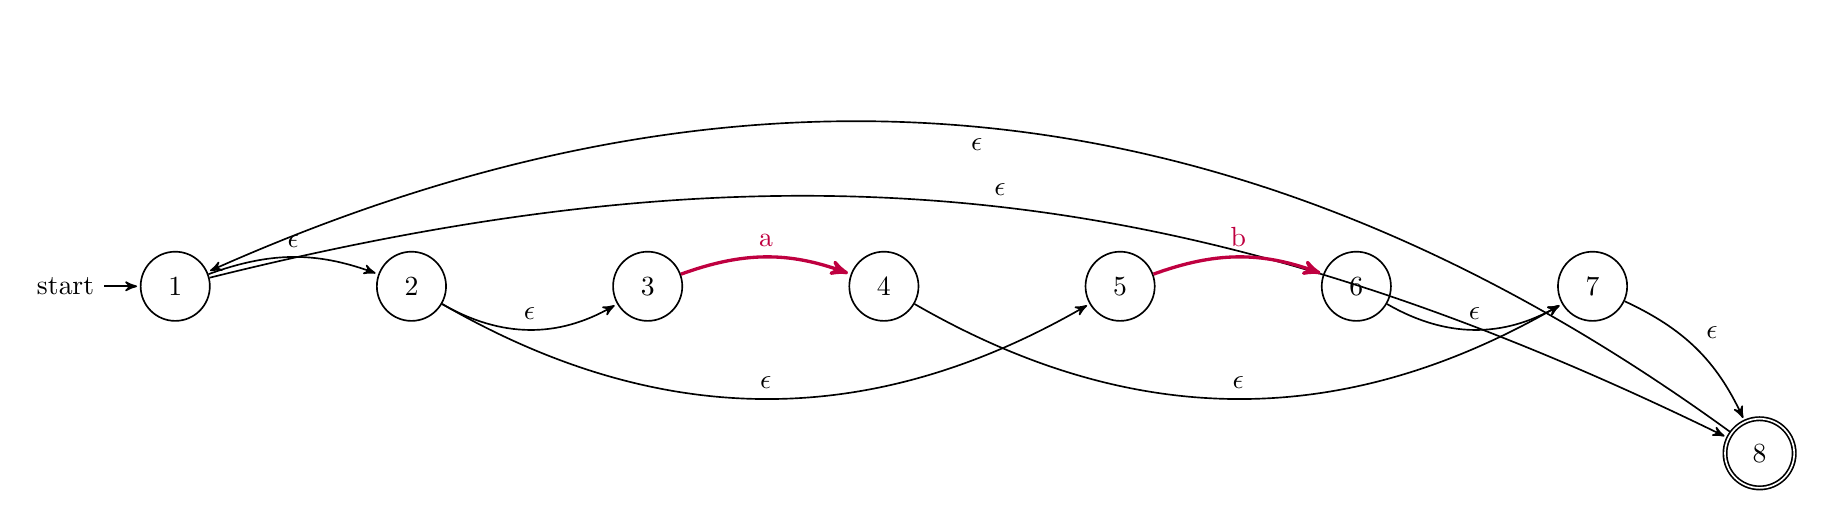
\begin{tikzpicture}
[->,>=stealth',shorten >=1pt,auto,node distance=3.0cm,semithick]\tikzstyle{every state}
=[fill=none,draw=black,text=black]
\node[initial,state] (1) {$1$};
\node[state] (2) [right of=1]  {$2$};
\node[state] (3) [right of=2]  {$3$};
\node[state] (4) [right of=3]  {$4$};
\node[state] (5) [right of=4]  {$5$};
\node[state] (6) [right of=5]  {$6$};
\node[state] (7) [right of=6]  {$7$};
\node[state, accepting] (8) [below right of=7] {$8$};

\path
(1) edge [bend left=20]  node {$\epsilon$} (2)

(8) edge [bend right]  node {$\epsilon$} (1)

(1) edge [bend left=20]  node {$\epsilon$} (8)

(7) edge [bend left=20]  node {$\epsilon$} (8)

(3) edge [purple, very thick, bend left=20]  node {a} (4)

(5) edge [purple, very thick, bend left=20]  node {b} (6)

(2) edge [bend right]  node {$\epsilon$} (3)

(2) edge [bend right]  node {$\epsilon$} (5)

(4) edge [bend right]  node {$\epsilon$} (7)

(6) edge [bend right]  node {$\epsilon$} (7)
;\end{tikzpicture}
\end{document}
